\documentclass[a4paper]{article}

\usepackage{myStyle}
\usepackage{commands}
\title{CD HA 02}

\begin{document}

\section{Invariante Unterräume}
Die Matrix
$$A_1 = \begin{pmatrix}
\frac{2}{5} & -\frac{6}{5} \\
-\frac{6}{5} & -\frac{7}{5}
\end{pmatrix}$$
hat die Eigenwerte $λ_1 = -2$ und $λ_2 = 1$ und es gilt
\begin{align*}
E^s = \ker (A - λ_1 I) &= \ker \begin{pmatrix}
12/5 & -6/5 \\ -6/5 & 3/5
\end{pmatrix} = \ker \begin{pmatrix}
1 & -6/12 \\ 1 & -3/6
\end{pmatrix}\\
&=\ker\begin{pmatrix}
1 & -6/12\\
0 & 0
\end{pmatrix} = \left\langle \begin{pmatrix}
1 \\ 12/6
\end{pmatrix} \right\rangle  
= \left\langle \begin{pmatrix}
1 \\ 2
\end{pmatrix} \right\rangle = \langle v_1 \rangle.
\end{align*}
Analog findet man
\begin{align*}
E^u = \ker (A -λ_2 I) = \langle v_2 \rangle = \left\langle \begin{pmatrix}
-2\\ 1
\end{pmatrix}\right\rangle.
\end{align*}

Die Matrix $A_2$ hat den zweifachen Eigenwert $-1$ mit dem zugehörigen stabilen Eigenraum 
$$
E^s = \left \langle \begin{pmatrix}
1\\ 2
\end{pmatrix}
\right\rangle$$
der Dimension 1.

Die Matrix $A_3$ hat die Eigenwerte 
\begin{align*}
    λ_1 &= 1 + 2i\\
    λ_2 &= 1 - 2i\\
    λ_3 &= -3
\end{align*}
mit den Eigenvektoren
$$
(v_1, v_2, v_3) =\begin{pmatrix}
-i & i & 0\\
1 & 1 & 0\\
0 & 0 & 1
\end{pmatrix}
$$
mit den Eigenräumen
\begin{align*}
E^s &= \langle v_3 \rangle &\text{(z-Achse stabil)}\\
E^u &= \langle v_1, v_2 \rangle
\end{align*}

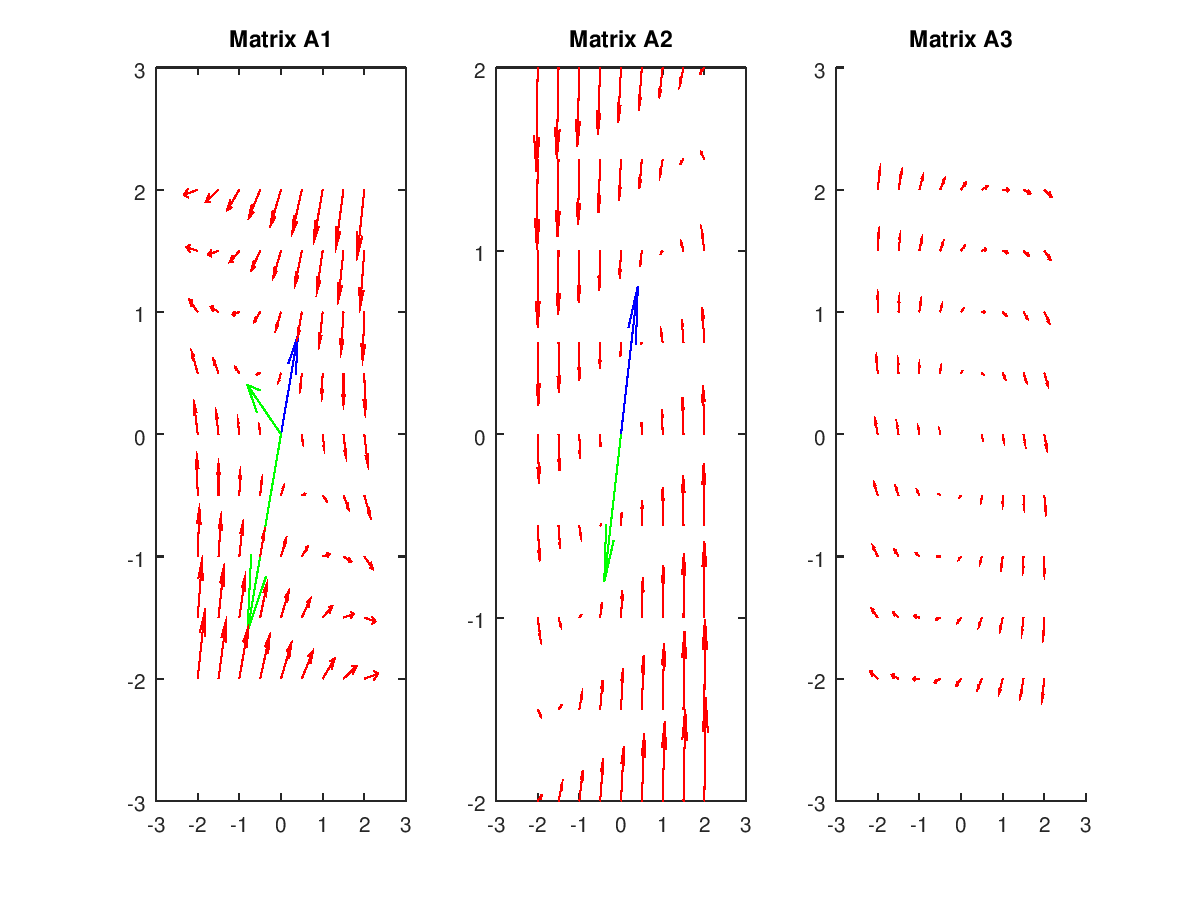
\includegraphics[height=5cm,width=0.9\textwidth]{imgs/cd_02_01.png}

% Aufgabe 2
\section{Eigenwerte Poincaré-Differential}
Es gilt zu zeigen, dass die Eigenwerte der Jacobischen der Poincaré-Abbildung unabhängig von der Wahl des transversalen Schnittes sind. 
Dabei nutzt man, dass ähnliche Matrizen die gleichen Eigenwerte haben.

Zunächst stellt man aber fest, dass verschiedene Poincaré-Abbildungen zueinander konjugiert sind. 
Es seien nämlich $Σ_1, Σ_2$ verschiedene transversale Schnitte durch zwei (nicht notwendig verschiedene) Punkte $p_1$ und $p_2$ auf dem periodischen Orbit $γ$. 
Seien $P_1, P_2$ die zugehörigen Poincaré-Abbildungen.
Dann gilt
$$p_2 = φ^s (p_1) \text{ für ein $0\le s < T$.}$$
Das Schnittlemma/Satz über implizite Funktionen liefert einen lokalen Diffeomorphismus
$$h\colon Σ_1 \to Σ_2, \; h(p_1) = p_2,$$
gegeben durch $h(ξ) = φ^{τ(ξ)} (ξ)$.
Damit gilt dann auch
$$P_2 \circ h = h\circ P_1.$$

Differentiation dieser Gleichung liefert
$$DP_2(p_2) \cdot Dh(p_1) = Dh(p_1) \cdot DP_1(p_1).$$
Da $h$ diffeomorph ist, können wir invertieren und mit $T = Dh(p_1)$ gilt:
$$DP_2(p_2) = T DP_1 (p_1) T^{-1},$$
also sind die Jacobi-Matrizen ähnlich und die Eigenwerte gleich, also unabhängig von der Wahl der Punkte auf dem Orbit und der transversalen Schnitte.

\section{Trivialer Floquet-Multiplikator}
Es sei $p=\overline x(0)$ für eine periodische Lösung. Wir wissen aus der Bemerkung nach der Definition der Floquet-Multiplikatoren, dass
$$Dφ^T(p) = e^{TR}$$
und somit sind die reicht es, zu zeigen, dass 1 ein Eigenwert von $DΦ^T(p)$ ist.

Dazu nutzt man die Flusseigenschaften und die Periodizität:
\begin{equation}
    \label{eqn:cd02_03}
    φ^t(p) = φ^T(φ^t(p)) = φ^t (φ^T(p)).
\end{equation}
Dann gilt
\begin{align*}
    f(p) &= f(\overline x(0)) = \dot x(t)|_{t=0} \\ 
    &=  \dt φ^t(p)|_{t=0} \\
    &\stackrel{\eqref{eqn:cd02_03}}= \dt\left( φ^T\circ φ^t (p)\right)|_{t=0}\\
    &=Dφ^T(p) \dot φ^0(p) \\
    &= Dφ^T(p) f(p)
    \end{align*}
und $f(p)$ ist Eigenvektor zum EW 1.
\end{document}